\documentclass[12pt,a4paper]{article}

% ─── Page Layout ───────────────────────────────────────────────────────────────
\usepackage[a4paper, margin=0.8in, headheight=14pt]{geometry}

% ─── Fonts (XeLaTeX) ───────────────────────────────────────────────────────────
\usepackage{fontspec}
\usepackage{unicode-math}
\setmainfont{TeX Gyre Pagella}
\setmonofont[Scale=0.88]{TeX Gyre Cursor}
\setmathfont{Latin Modern Math}

% ─── Packages ──────────────────────────────────────────────────────────────────
\usepackage{xcolor}
\usepackage{colortbl}
\usepackage{titlesec}
\usepackage{enumitem}
\usepackage{tabularx}
\usepackage{booktabs}
\usepackage{array}
\usepackage{amsmath}
\usepackage{tikz}
\usetikzlibrary{shapes.geometric, arrows.meta, positioning, calc, fit, decorations.pathreplacing}
\usepackage{tcolorbox}
\tcbuselibrary{skins, breakable}
\usepackage{hyperref}
\usepackage{fancyhdr}
\usepackage{graphicx}
\usepackage{microtype}
\hyphenpenalty=10000
\exhyphenpenalty=10000
\sloppy
\usepackage{caption}
\usepackage{setspace}
\usepackage{multirow}
\usepackage{tocloft}

% ─── Q&A helper ────────────────────────────────────────────────────────────────
\newcommand{\Q}[1]{\textbf{#1}\par\noindent\ignorespaces}

% ─── Colour Palette ────────────────────────────────────────────────────────────
\definecolor{myred}{RGB}{196,30,58}
\definecolor{mydark}{RGB}{30,30,50}
\definecolor{mygreen}{RGB}{14,120,80}
\definecolor{myteal}{RGB}{0,130,140}
\definecolor{myamber}{RGB}{180,100,0}
\definecolor{mypurple}{RGB}{100,30,160}
\definecolor{mygray}{RGB}{246,247,249}
\definecolor{mgframe}{RGB}{180,185,200}
\definecolor{watermark}{RGB}{145,150,170}
\definecolor{hdrred}{RGB}{250,232,235}
\definecolor{hdrgreen}{RGB}{220,244,233}
\definecolor{hdrteal}{RGB}{220,242,244}
\definecolor{hdramber}{RGB}{253,242,215}
\definecolor{hdrpurple}{RGB}{238,228,255}
\definecolor{hdrgray}{RGB}{238,240,245}
\definecolor{rowalt}{RGB}{250,251,253}

% ─── Section Formatting ────────────────────────────────────────────────────────
\titleformat{\section}
  {\large\bfseries\color{myred}}{\thesection.}{0.5em}{}
  [\vspace{1pt}{\color{myred}\rule{\linewidth}{0.8pt}}]
\titleformat{\subsection}
  {\normalsize\bfseries\color{myteal}}{\thesubsection}{0.5em}{}
\titlespacing*{\section}{0pt}{18pt}{7pt}
\titlespacing*{\subsection}{0pt}{11pt}{4pt}

% ─── Paragraph ─────────────────────────────────────────────────────────────────
\setlength{\parindent}{0pt}
\setlength{\parskip}{4pt}

% ─── TOC Styling ───────────────────────────────────────────────────────────────
\renewcommand{\cfttoctitlefont}{\large\bfseries\color{myred}}
\renewcommand{\cftaftertoctitle}{\par\noindent{\color{myred}\rule{\linewidth}{0.8pt}}}
\setlength{\cftbeforetoctitleskip}{0pt}
\setlength{\cftaftertoctitleskip}{6pt}
\renewcommand{\cftsecfont}{\normalsize\bfseries\color{mydark}}
\renewcommand{\cftsecpagefont}{\normalsize\bfseries\color{mydark}}
\renewcommand{\cftsecleader}{\cftdotfill{\cftdotsep}}
\setlength{\cftbeforesecskip}{7pt}
\renewcommand{\cftsubsecfont}{\small\color{mydark}}
\renewcommand{\cftsubsecpagefont}{\small\color{mydark}}
\setlength{\cftbeforesubsecskip}{3pt}
\setlength{\cftsubsecindent}{1.4em}

% ─── Table helpers ─────────────────────────────────────────────────────────────
\renewcommand{\arraystretch}{1.45}
\setlength{\tabcolsep}{6pt}
\arrayrulecolor{mydark}
\newcolumntype{B}[1]{>{\small\bfseries\raggedright\arraybackslash}m{#1}}
\newcolumntype{Y}{>{\small\raggedright\arraybackslash}X}
\renewcommand{\tabularxcolumn}[1]{m{#1}}

% ─── Header / Footer ───────────────────────────────────────────────────────────
\pagestyle{fancy}
\fancyhf{}
\fancyhead[L]{\small\color{myred}\textbf{PE-EC701A}\;\color{mydark}--- Microwave Theory and Technique}
\fancyhead[R]{\small\color{myteal}\textbf{Module 4 Notes}}
\fancyfoot[C]{\small\color{mydark}\thepage}
\fancyfoot[R]{\small\color{watermark}\textit{\copyright\ Biraj}}
\renewcommand{\headrulewidth}{0.5pt}
\renewcommand{\footrulewidth}{0.3pt}

% ─── Hyperref ──────────────────────────────────────────────────────────────────
\hypersetup{
  colorlinks=true, linkcolor=myteal, urlcolor=myteal,
  pdfauthor={Biraj Sarkar},
  pdftitle={PE-EC701A --- Module 4 Notes}
}

% ─── tcolorbox styles ──────────────────────────────────────────────────────────
\tcbset{
  tikzbox/.style={
    colback=mygray, colframe=mgframe, boxrule=0.6pt, arc=4pt,
    left=8pt, right=8pt, top=6pt, bottom=6pt,
    colbacktitle=mgframe, coltitle=mydark,
    fonttitle=\small\bfseries
  },
  defbox/.style={
    colback=hdrgreen, colframe=mygreen, boxrule=0.8pt, arc=4pt,
    left=9pt, right=9pt, top=6pt, bottom=6pt,
    colbacktitle=mygreen, coltitle=white,
    fonttitle=\small\bfseries
  },
  formulabox/.style={
    colback=hdrteal, colframe=myteal, boxrule=0.8pt, arc=4pt,
    left=9pt, right=9pt, top=7pt, bottom=7pt,
    colbacktitle=myteal, coltitle=white,
    fonttitle=\small\bfseries
  },
  examplebox/.style={
    colback=hdramber, colframe=myamber, boxrule=0.8pt, arc=4pt,
    left=9pt, right=9pt, top=6pt, bottom=6pt,
    colbacktitle=myamber, coltitle=white,
    fonttitle=\small\bfseries
  },
  masonbox/.style={
    colback=hdrpurple, colframe=mypurple, boxrule=0.8pt, arc=4pt,
    left=9pt, right=9pt, top=6pt, bottom=6pt,
    colbacktitle=mypurple, coltitle=white,
    fonttitle=\small\bfseries
  },
  exambox/.style={
    colback=hdrpurple, colframe=mypurple, boxrule=1pt, arc=5pt,
    left=10pt, right=10pt, top=8pt, bottom=8pt,
    colbacktitle=mypurple, coltitle=white,
    fonttitle=\bfseries,
    breakable, title after break={\textbf{Frequently Asked / Viva Questions (contd.)}}}
}
% Make all boxes breakable across pages
\tcbset{breakable}

% ─── TikZ styles ───────────────────────────────────────────────────────────────
\tikzset{
  block/.style={rectangle, draw=myteal, fill=hdrteal,
    text width=2.4cm, align=center, minimum height=0.95cm,
    font=\small, rounded corners=3pt, line width=0.7pt},
  redblock/.style={rectangle, draw=myred, fill=hdrred,
    text width=2.4cm, align=center, minimum height=0.95cm,
    font=\small, rounded corners=3pt, line width=0.7pt},
  netnode/.style={rectangle, draw=myteal, fill=hdrteal,
    text width=1.5cm, align=center, minimum height=0.8cm,
    font=\small, rounded corners=3pt, line width=0.7pt},
  sumjunc/.style={circle, draw=myamber, fill=hdramber,
    minimum size=0.62cm, font=\small, line width=0.8pt},
  snode/.style={circle, draw=mypurple, fill=hdrpurple,
    minimum size=0.55cm, font=\footnotesize, line width=0.7pt},
  arrow/.style={-Stealth, thick, color=mydark},
  redarrow/.style={-Stealth, thick, color=myred},
  line/.style={thick, color=mydark}
}

% ═══════════════════════════════════════════════════════════════════════════════
\begin{document}
% ═══════════════════════════════════════════════════════════════════════════════

\begin{center}
  {\LARGE\bfseries\color{myred} PE-EC701A --- Microwave Theory and Technique}\\[5pt]
  {\normalsize\color{mydark} Semester VII \quad$\bullet$\quad 3L:0T:0P \quad$\bullet$\quad 3 Credits}\\[3pt]
  {\normalsize\color{myteal}\textbf{Module 4 Exam Notes: Microwave Network Analysis}}\\[3pt]
  {\small\color{mydark} CGEC \;$|$\; B.Tech ECE (2023--27) \;$|$\; \textit{Biraj Sarkar}}
\end{center}
\vspace{2pt}
\noindent{\color{myred}\rule{\linewidth}{1.5pt}}
\vspace{2pt}

\hypersetup{linkcolor=mydark}
\tableofcontents
\hypersetup{linkcolor=myteal}
\newpage

% ===============================================================================
\section{Equivalent Voltages and Currents for Non-TEM Lines}
% ===============================================================================

In waveguides supporting TE or TM modes, the physical voltage and current are not uniquely defined because the electric and magnetic fields vary spatially across the guide cross-section. 

\begin{tcolorbox}[defbox]
\textbf{Equivalent Voltage and Current:} Normalized wave quantities defined such that their ratio equals the wave impedance ($Z_w$) and their product represents the power flow ($P$) down the waveguide. They allow waveguides to be analyzed using standard transmission line theory.
\end{tcolorbox}

Let $E_t$ and $H_t$ be the transverse electric and magnetic fields. The equivalent voltage $V(z)$ and current $I(z)$ are defined as:
\begin{align}
  V(z) &= K_V \iint_{S} E_t \cdot e_n \,dS \\
  I(z) &= K_I \iint_{S} H_t \cdot h_n \,dS
\end{align}
Where $e_n, h_n$ are transverse vector mode functions. The normalization is chosen such that:
\begin{equation}
  P = \frac{1}{2} \text{Re}(V I^*) \quad \text{and} \quad \frac{V}{I} = Z_w
\end{equation}

% ===============================================================================
\section{Scattering (S) Parameters}
% ===============================================================================

At high frequencies (microwave range), traditional low-frequency network parameters such as Impedance ($Z$), Admittance ($Y$), and Transmission ($ABCD$) parameters become extremely difficult to measure.

\subsection{Why S-Parameters are Preferred at Microwaves}
\begin{itemize}[leftmargin=*, itemsep=4pt]
  \item \textbf{No Open/Short Circuit Requirements:} Measuring $Z$ and $Y$ parameters requires establishing perfect open and short circuits at the device terminals. At GHz frequencies, lead inductance and stray capacitance make perfect open/shorts impossible to realize.
  \item \textbf{Device Protection:} Creating a short circuit on active microwave devices (like Gunn diodes or high-frequency transistors) can cause them to become unstable and self-oscillate, potentially damaging the device.
  \item \textbf{Matched Terminations:} S-parameters are measured using \textbf{matched loads} (typically $50\,\Omega$). Matched loads are easy to construct at high frequencies and prevent signal reflections.
  \item \textbf{Direct Link to Wave Quantities:} S-parameters relate directly to incident and reflected power waves, which are easily measured using directional couplers.
\end{itemize}

\subsection{S-Parameter Mathematical Definition}
Consider an $N$-port microwave network. At each port $i$, we define normalized incident and reflected wave variables $a_i$ and $b_i$:

\begin{tcolorbox}[tikzbox, title={N-Port Microwave Network Wave Variables}]
\centering
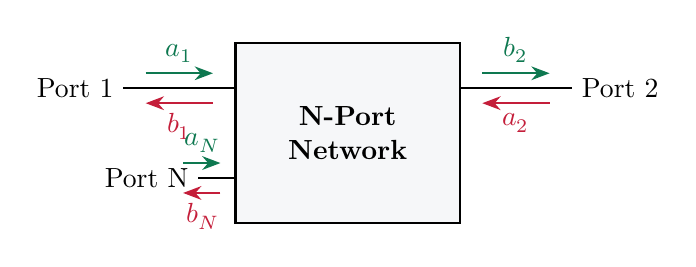
\begin{tikzpicture}[scale=0.95]
  % Central network box
  \draw[thick, fill=mygray] (-1.5,-1.2) rectangle (1.5,1.2);
  \node[font=\bfseries, align=center] at (0,0) {N-Port\\Network};
  
  % Port 1
  \draw[thick] (-3,0.6) -- (-1.5,0.6);
  \node[left] at (-3,0.6) {Port 1};
  \draw[-Stealth, color=mygreen, thick] (-2.7,0.8) -- (-1.8,0.8) node[midway, above] {$a_1$};
  \draw[-Stealth, color=myred, thick] (-1.8,0.4) -- (-2.7,0.4) node[midway, below] {$b_1$};
  
  % Port 2
  \draw[thick] (1.5,0.6) -- (3,0.6);
  \node[right] at (3,0.6) {Port 2};
  \draw[-Stealth, color=mygreen, thick] (1.8,0.8) -- (2.7,0.8) node[midway, above] {$b_2$};
  \draw[-Stealth, color=myred, thick] (2.7,0.4) -- (1.8,0.4) node[midway, below] {$a_2$};
  
  % Port N
  \draw[thick] (-2,-0.6) -- (-1.5,-0.6);
  \node[left] at (-2,-0.6) {Port N};
  \draw[-Stealth, color=mygreen, thick] (-2.2,-0.4) -- (-1.7,-0.4) node[midway, above] {$a_N$};
  \draw[-Stealth, color=myred, thick] (-1.7,-0.8) -- (-2.2,-0.8) node[midway, below] {$b_N$};
\end{tikzpicture}
\end{tcolorbox}

\begin{tcolorbox}[formulabox, title={\textbf{Scattering Parameter Relations}}]
The wave variables $a_i$ (incident) and $b_i$ (reflected) are related to port voltages $V_i$, currents $I_i$, and characteristic impedance $Z_0$ by:
\begin{align}
  a_i &= \frac{V_i + I_i Z_0}{2\sqrt{Z_0}} \quad (\text{incident wave}) \\
  b_i &= \frac{V_i - I_i Z_0}{2\sqrt{Z_0}} \quad (\text{reflected wave})
\end{align}
The linear relationship between the waves is expressed in matrix form as:
\begin{equation}
  [b] = [S][a]
\end{equation}
For a 2-port network:
\begin{equation}
  \begin{bmatrix} b_1 \\ b_2 \end{bmatrix} = \begin{bmatrix} S_{11} & S_{12} \\ S_{21} & S_{22} \end{bmatrix} \begin{bmatrix} a_1 \\ a_2 \end{bmatrix}
\end{equation}
Where:
\begin{itemize}[leftmargin=1.5em, itemsep=1.5pt]
  \item[] $S_{ii} = \left. \frac{b_i}{a_i} \right|_{a_k=0 \text{ for } k \ne i}$ is the reflection coefficient at port $i$ when all other ports are matched.
  \item[] $S_{ij} = \left. \frac{b_i}{a_j} \right|_{a_k=0 \text{ for } k \ne j}$ is the transmission coefficient from port $j$ to port $i$ under matched termination.
\end{itemize}
\end{tcolorbox}

% ===============================================================================
\section{Properties of the S-Matrix}
% ===============================================================================

The S-matrix possesses key mathematical properties governed by reciprocity and conservation of energy.

\subsection{Symmetric Property for Reciprocal Networks}
A network is reciprocal if the transmission of energy from port $i$ to port $j$ is identical to transmission from $j$ to $i$.
\begin{tcolorbox}[defbox]
\textbf{Symmetric Property:} The scattering matrix of a reciprocal network is symmetric.
\begin{equation}
  [S]^T = [S] \quad \implies \quad S_{ij} = S_{ji}
\end{equation}
\end{tcolorbox}

\subsubsection{Derivation of the Reciprocal Property}
For a reciprocal network, the impedance matrix $[Z]$ is symmetric:
\begin{equation*}
  [Z]^T = [Z]
\end{equation*}
The relationship between S-parameters and Z-parameters (normalized to $Z_0 = 1$) is:
\begin{equation}
  [S] = ([Z] - [I])([Z] + [I])^{-1}
\end{equation}
Taking the transpose of both sides:
\begin{align*}
  [S]^T &= \left[ ([Z] - [I])([Z] + [I])^{-1} \right]^T \\
  &= \left( ([Z] + [I])^{-1} \right)^T \cdot ([Z] - [I])^T \\
  &= \left( ([Z] + [I])^T \right)^{-1} \cdot ([Z]^T - [I]^T)
\end{align*}
Since $[Z]^T = [Z]$ and the identity matrix is symmetric ($[I]^T = [I]$):
\begin{equation*}
  [S]^T = ([Z] + [I])^{-1} ([Z] - [I])
\end{equation*}
Since matrices of the form $([Z] \pm [I])$ commute:
\begin{equation*}
  ([Z] + [I])^{-1} ([Z] - [I]) = ([Z] - [I]) ([Z] + [I])^{-1} = [S]
\end{equation*}
Thus, we prove:
\begin{equation}
  [S]^T = [S] \quad \text{(Q.E.D.)}
\end{equation}

\subsection{Unitary Property for Lossless Networks}
In a lossless network, no real power is dissipated; the total power entering the network must equal the total power leaving it.
\begin{tcolorbox}[defbox]
\textbf{Unitary Property:} The S-matrix of a lossless network is unitary.
\begin{equation}
  [S]^{*, T} [S] = [I] \quad \text{or} \quad [S]^\dagger [S] = [I]
\end{equation}
\end{tcolorbox}

\subsubsection{Derivation of the Lossless Property}
The total power entering an $N$-port network is the sum of incident powers:
\begin{equation*}
  P_{in} = \frac{1}{2} \sum_{i=1}^N |a_i|^2 = \frac{1}{2} [a]^{*, T} [a]
\end{equation*}
The total power leaving the network is the sum of reflected powers:
\begin{equation*}
  P_{out} = \frac{1}{2} \sum_{i=1}^N |b_i|^2 = \frac{1}{2} [b]^{*, T} [b]
\end{equation*}
Since the network is lossless, conservation of energy dictates $P_{in} = P_{out}$:
\begin{equation*}
  [a]^{*, T} [a] = [b]^{*, T} [b]
\end{equation*}
Substituting $[b] = [S][a]$ and taking its conjugate transpose $[b]^{*, T} = [a]^{*, T} [S]^{*, T}$:
\begin{equation*}
  [a]^{*, T} [a] = [a]^{*, T} [S]^{*, T} [S] [a]
\end{equation*}
This equation must hold for any arbitrary incident wave vector $[a]$. Hence:
\begin{equation}
  [S]^{*, T} [S] = [I] \quad \text{(Q.E.D.)}
\end{equation}

% ===============================================================================
% MANDATORY QUICK REVISION PAGE
% ===============================================================================
\newpage
\begin{center}
  {\large\bfseries\color{myred} Quick Revision --- Module IV}\\[3pt]
  {\small\color{mydark} Microwave Network Analysis $|$ PE-EC701A}
\end{center}
\noindent{\color{myred}\rule{\linewidth}{1.2pt}}
\vspace{4pt}

\begin{tcolorbox}[formulabox, title={\textbf{Key Formulas at a Glance}}]
\renewcommand{\arraystretch}{1.3}
\begin{tabularx}{\linewidth}{B{4.5cm} X}Incident wave variable  & $a_i = \frac{V_i + I_i Z_0}{2\sqrt{Z_0}}$ \\[4pt]
Reflected wave variable  & $b_i = \frac{V_i - I_i Z_0}{2\sqrt{Z_0}}$ \\[4pt]
Reciprocal condition    & $[S]^T = [S] \quad \implies S_{ij} = S_{ji}$ \\[4pt]
Lossless condition      & $[S]^{*, T} [S] = [I] \quad \implies \sum_{k=1}^N S_{ki}^* S_{kj} = \delta_{ij}$ \\[4pt]
Reflection \& VSWR      & $S_{11} = \Gamma = \frac{\text{VSWR}-1}{\text{VSWR}+1}$
\end{tabularx}
\tcbset{colbacktitle=mygreen, coltitle=white}
\end{tcolorbox}

\begin{tcolorbox}[defbox, title={\textbf{One-Line Definitions}}]
\begin{itemize}[leftmargin=*, itemsep=2.5pt, topsep=0pt]
  \item \textbf{S-Parameters:} Network parameters relating incident and reflected voltage waves.
  \item \textbf{Reciprocal Network:} A passive network where transmission coefficients are independent of propagation direction.
  \item \textbf{Lossless Network:} A network that conserves RF power, having zero internal power dissipation.
  \item \textbf{Unitary Matrix:} A complex matrix whose conjugate transpose is also its inverse.
  \item \textbf{Insertion Loss:} The attenuation of a signal passing through a network, given by $-20 \log_{10}|S_{ji}|$ dB.
  \item \textbf{Return Loss:} A measure of reflection mismatch at a port, given by $-20 \log_{10}|S_{ii}|$ dB.
  \item \textbf{Matched Termination:} Connecting a load equal to the characteristic impedance, preventing reflection.
\end{itemize}
\end{tcolorbox}

\begin{tcolorbox}[exambox, title={\textbf{Frequently Asked / Viva Questions}}]
\begin{enumerate}[topsep=0pt, label=\textbf{Q\arabic*.}, itemsep=5pt]
  \item \Q{Why are Z and Y parameters not suitable for microwave frequencies?}
    Because they require open and short circuit terminations. At microwave frequencies, parasitics make open/shorts impossible, and shorts can damage active devices.
  \item \Q{What is the physical meaning of $S_{11}$ and $S_{21}$?}
    $S_{11}$ is the input reflection coefficient when port 2 is matched. $S_{21}$ is the forward transmission coefficient from port 1 to port 2 when port 2 is matched.
  \item \Q{State the unitary property of the S-matrix in summation form.}
    For a lossless network, $\sum_{k=1}^N |S_{ki}|^2 = 1$ (unity relation) and $\sum_{k=1}^N S_{ki}^* S_{kj} = 0$ for $i \ne j$ (zero relation).
  \item \Q{Prove that a 1-port network with a matched load has $S_{11} = 0$.}
    A matched load absorbs all incident energy, generating zero reflected wave ($b_1 = 0$), so $S_{11} = b_1/a_1 = 0$.
  \item \Q{What is the relationship between S-parameters and ABCD parameters?}
    ABCD parameters relate input voltage and current to output voltage and current. They are cascading parameters, unlike S-parameters which relate incident/reflected waves.
  \item \Q{Why are S-parameters measured relative to a specific reference impedance (usually $50\,\Omega$)?}
    Because wave variables $a$ and $b$ are normalized to $\sqrt{Z_0}$. Changing $Z_0$ changes the values of the S-parameters.
  \item \Q{What does a return loss of $\infty$ dB represent?}
    It represents a perfect match ($S_{11} = 0$), where no signal is reflected back.
  \item \Q{How do you check if an S-matrix represents a physical, passive network?}
    The magnitude of all elements must be less than or equal to one ($|S_{ij}| \le 1$), and the network must not generate net power (the eigenvalues of $[S]^{*,T}[S]$ must be $\le 1$).
  \item \Q{What is the relation between S-parameters and VSWR?}
    $\text{VSWR} = \frac{1 + |S_{ii}|}{1 - |S_{ii}|}$.
  \item \Q{Under what conditions is the ABCD matrix preferred over the S-matrix?}
    When cascading multiple microwave networks in series, because the overall ABCD matrix is simply the product of individual ABCD matrices ($[ABCD]_{\text{total}} = [A] \cdot [B] \dots$).
  \item \Q{What is equivocation in the context of network transmission?}
    It is the power lost or diverted due to reflection and mismatch at network junctions.
  \item \Q{Why is the S-matrix symmetric for reciprocal networks?}
    Because the underlying electromagnetic materials are isotropic, yielding symmetric impedance ($[Z]$) and admittance ($[Y]$) matrices, which mathematically maps to $[S]^T = [S]$.
\end{enumerate}
\tcbset{colbacktitle=mgframe, coltitle=mydark}
\end{tcolorbox}

\begin{tcolorbox}[tikzbox, title={Comparison of Z, Y, ABCD, and S-Parameters}]
\renewcommand{\arraystretch}{1.4}
\par\noindent
{\renewcommand{\arraystretch}{1.65}%
\begin{tabularx}{\linewidth}{|B{2.8cm}|Y|Y|Y|}\hline
\textbf{Parameters} & \textbf{Independent Variables} & \textbf{Dependent Variables} & \textbf{Terminations Required} \\[4pt]
\hline
\textbf{Z Parameters} & Currents ($I_1, I_2$) & Voltages ($V_1, V_2$) & Open Circuit ($I = 0$) \\[4pt]
\hline
\textbf{Y Parameters} & Voltages ($V_1, V_2$) & Currents ($I_1, I_2$) & Short Circuit ($V = 0$) \\[4pt]
\hline
\textbf{ABCD Params} & Output variables ($V_2, -I_2$) & Input variables ($V_1, I_1$) & Open / Short depending on parameter \\[4pt]
\hline
\textbf{S Parameters} & Incident Waves ($a_1, a_2$) & Reflected Waves ($b_1, b_2$) & Matched Termination ($a = 0$) \\[4pt]
\hline
\end{tabularx}
}
\end{tcolorbox}

\end{document}
